\textcolor{red}{\section{Real hardware implementation}\label{EDCA}}

We confirmed experimentally the simulations with a testbed of real prototypes. This phase was mandatory to check whether the behaviour of the system is still correct in the presence of unexpected phenomena like excessive channel noise, or technical limitations of the hardware like imperfect node synchronisation; and to verify the implementation feasibility of the halving technique with a real time horizon.

As CSMA/ECA$_{\text{Hys}}$ works with the standard 802.11 PHY, we do not need the flexibility offered by complex development kits based on FPGAs like the WARP boards (add citation): any architecture that allows a customisation of the channel access delay would fit our requirements. For this reason we chose a widely available 802.11bg WNIC from Broadcom: like many other cards, its behaviour is ruled by a firmware code that controls the underlying hardware (including the radio, carrier sense and FIFOs) in real time. In particular we used the BRCM4318KBFG PCI card as it is supported by the OpenFWWF~\cite{OpenFWWF} open--source firmware, an alternative to the original code from the manufacturer that has been recently considered as development platform in several research projects (add citations). 
Thanks to the extremely low price of this card (refurbish devices are widely available for less than $10\$$ each), it is possible to run experiments with very large testbeds: in our case we used 25 PC-Engines Alix 2d2 nodes running Linux kernel 2.6.32 as stations and a more powerful computer with the same kernel as access point, all nodes being equipped with the aforementioned WNIC.

We built on the DCF protocol implemented in OpenFWWF and we adapted the firmware to create the basic collision free schedule as described in Algorithm \ref{alg:CSMA_CA}. The modification was straightforward: for every transmitted data frame, in fact, the firmware sets an ACK-time-out alarm. Later, both at the expiration of the timer or when the acknowledgment frame is received, it executes handler labelled {\tt tx\_contention\_params\_update}. Here we update the contention window value {\tt STATE\_CW} according to the success/failure outcome of the transmission attempt as in the algorithm. To embed the stickiness feature into the algorithm, we add a {\tt STATE} to the system that can be either {\tt STATE\_DETERMINISTIC} or {\tt STATE\_RANDOM} and a {\tt STICKINESS} counter that we reset each time we have a success and decrement when failing: when it gets to zero we enter the random state. Upon a successful delivery we unconditionally enter the deterministic state and we reset the stickiness counter to {\tt DEFAULT\_STICKINESS}. Setting this last parameter to zero lets the system operate without the stickiness feature.

To introduce the halving mechanism we added a bitmap for monitoring the state of every single slot after a successful transmission. To index the current slot in the bitmap we use on the hardware register {\tt SPR\_IFS\_BKOFFDELAY} which counts how many slots have still to come before the next transmission and decrements once per idle slot as requested by the DCF procedure: the idea is to start with an empty bitmap and mark those slots for which the countdown procedure was interrupted. To avoid spurious detection, instead of continuously checking the state of the channel, we rely on the execution of the {\tt rx\_plcp} handler that is called each time a valid PLCP is detected. When this happens, we implicitely know that the backoff counter has been frozen since at least $20\mu s$, that is the time between the first repetitions of the short training sequence have been detected and the complete decoding of the PLCP signal data: in any case the current slot has to be marked as busy. We have the option to keep filling the bitmap for up to {\tt BITMAP\_ROUND\_BUILD} consecutive successful deliveries before checking if the central slot in the bitmap is available, and, in case halving the deterministic schedule.

	\begin{figure}[tb]
		\centering
		\includegraphics[width=0.7\linewidth,angle=-90]{figures/tonFigs/throughput-sat-SR-IMPLEMENTATION.eps}
		\caption{Average aggregated throughput for a saturated network. Real hardware implementation results}
		\label{fig:throughputImplementation}
	\end{figure}
	
	\begin{figure}[tb]
		\centering
		\includegraphics[width=0.7\linewidth,angle=-90]{figures/tonFigs/losses-sat-SR-IMPLEMENTATION.eps}
		\caption{Average percentage of losses for a saturated network. Real hardware implementation results}
		\label{fis:lossesImplementation}
	\end{figure}


%\textcolor{red}{\it maybe we could add a figure to explain of the bitmap is filled}
%
%\textcolor{red}{The new section should assume that the implementation has already been done. Further, it should overview:}
%
%\textcolor{red}{\begin{itemize}
%	\item Why do we need it?
%	\item Are there other alternatives?
%	\item How does it do what it does? (I think the explanation of the CF-MAC paper should suffice).
%	\item You can refer to the firmware implementation as CSMA/ECA$_{\text{Hys}}$ with Schedule Halving and dynamic Stickiness. I will define it before this section.
%\end{itemize}}
%
%\textcolor{red}{Obviously this will be a first revision. I leave the rest of the section untouched, we will erase/modify it later. Thanks in advance.}
%
%The implementation of CSMA/ECA$_{\text{Hys+FS}}$ should be carried out at a firmware level due to the tight timing constrains related to the backoff procedure. There are several alternatives to modify the backoff operation in WNICs, either using open firmware like OpenFWWF~\cite{OpenFWWF} or through Field Programmable Gate Arrays (FPGA).
%
%Although the FPGA option would in theory provide the strict timing requirements, the associated costs and difficulty are greater than the OpenFWWF alternative. OpenFWWF provides an open CSMA/CA firmware for a specific model of Broadcom WNICs' chipset, so the resulting firmware can be uploaded and tested in real commercial hardware. 
%
%By making the modifications represented in Algorithm~\ref{alg:CSMA_ECA}, a proof-of-concept prototype of CSMA/ECA was built using comercial hardware~\cite{ECA-DEMO-INFOCOM14, sanabria2013prototyping, BECA-test}. The prototype was able to create a collision-free schedule among a reduced number of contenders using big deterministic backoffs (such as $128$ or $256$ slots). Nevertheless, clock drift, imprecise timing~\cite{bianchi2007experimental} and other prototyping non-idialities prevented the construction of a collision-free schedule when using a small deterministic backoff or dynamic rate adaptation algorithms, like Minstrel~\cite{minstrel}.
%
%Although the timing inaccuracy issues were identified and leveraged to prototype a similar protocol in real hardware~\cite{CF-MAC}, further development on the prototype is being carried out in order to incorporate Hysteresis and Fair Share.